Dalam pengembangan aplikasi berbasis \textit{website}, \textit{website} tidak hanya dituntut untuk memiliki tampilan yang informatif dan interaktif, tetapi juga memerlukan standar keamanan serta keandalan. Aplikasi yang terhubung langsung ke internet rentan terhadap berbagai ancaman siber, seperti pencurian data sensitif maupun manipulasi sistem, yang pada akhirnya dapat mengganggu operasional bisnis. Bagi suatu organisasi, risiko ini meningkat ketika data internal yang sifatnya sensitif harus diakses oleh aplikasi \textit{website} yang bersifat publik.

Salah satu pendekatan untuk mengurangi risiko tersebut adalah dengan memisahkan komponen publik dari lingkungan internal organisasi. Melalui pengaturan ini, aplikasi \textit{website} dapat difungsikan sebagai antarmuka publik yang menampilkan data dan konten, sedangkan aplikasi internal yang menyimpan logika bisnis dan data sensitif tetap berada pada lingkungan yang lebih terbatas. Langkah ini mengurangi akses eksternal langsung ke sumber data internal, sehingga memperkuat lapisan keamanan dan mengurangi paparan terhadap ancaman siber.

Meskipun demikian, tantangan lain muncul ketika sebuah organisasi memiliki beragam aplikasi internal yang menyuplai data ke aplikasi \textit{website}. Kondisi ini sering menimbulkan kompleksitas dalam integrasi data, pengelolaan konten, serta sinkronisasi informasi, karena masing-masing aplikasi internal dapat memiliki skema data, format, atau aturan bisnis yang berbeda. Tanpa mekanisme integrasi yang terpusat, menjaga konsistensi konten antara aplikasi internal dan aplikasi \textit{website} menjadi sulit, sehingga berdampak pada kualitas informasi yang disajikan kepada pengguna.

Untuk mengatasi tantangan tersebut, dalam tugas akhir ini dikembangkan sebuah \textit{generator} konten \textit{website} berbasis API yang dirancang dengan fokus pada keamanan serta keandalan. Sistem ini tidak hanya mengandalkan templat statis, tetapi juga memanfaatkan data aplikasi web dan data yang diambil secara terkini dari aplikasi internal. Dengan demikian, proses \textit{generate content website} selalu mengacu pada data paling mutakhir, sekaligus memastikan data sensitif tidak terekspos secara langsung. Dari sisi keandalan, sistem mengimplementasikan mekanisme sinkronisasi yang berlangsung dalam dua tahap:  
(1) Sinkronisasi data dari aplikasi internal ke aplikasi\textit{website} dilakukan pada saat proses \textit{generate website}, sehingga konten pada \textit{website} menggunakan data paling mutahir.
(2) Sinkronisasi data dari \textit{website} ke aplikasi internal dilakukan secara terjadwal, di mana data yang akan disinkronkan, terlebih dahulu diverifikasi berdasarkan templat dan aturan yang tersimpan pada basis data.

Dengan pendekatan ini, organisasi dapat membangun aplikasi \textit{website} yang aman dan handal tanpa mengorbankan perlindungan data internal. Seluruh proses integrasi dan sinkronisasi dikelola secara terkontrol melalui API \textit{generator} konten \textit{website}.

Secara umum, alur kerja sistem ini dapat dilihat pada Gambar \ref{fig:GambaranUmum}. Prosesnya mencakup tiga langkah utama:
\begin{enumerate}
    
    \item \textbf{Pembangunan aplikasi \textit{website}:} \textit{Generator} (G) membangun aplikasi \textit{website} (AW) berdasarkan templat yang tersimpan di Basis Data Templat (T), data aplikasi \textit{website} yang sudah ada aplikasi internal (AI), serta data asli aplikasi internal (AI) yang terkini.
    
    \item \textbf{Sinkronisasi data terjadwal:} \textit{Sinkronisator} (S) secara berkala mengambil data dari aplikasi \textit{website} (AW), memvalidasinya berdasarkan aturan yang ada di basis data templat (T), lalu mengirimkannya kembali ke aplikasi internal (AI).
    
    \item \textbf{Akses aman oleh pengguna:} Pengguna mengakses aplikasi \textit{website} (AW) melalui mekanisme \textit{Single Sign-On} (SSO) demi menjaga keamanan akses.
    
\end{enumerate}

\begin{figure}[H]
    \centering
    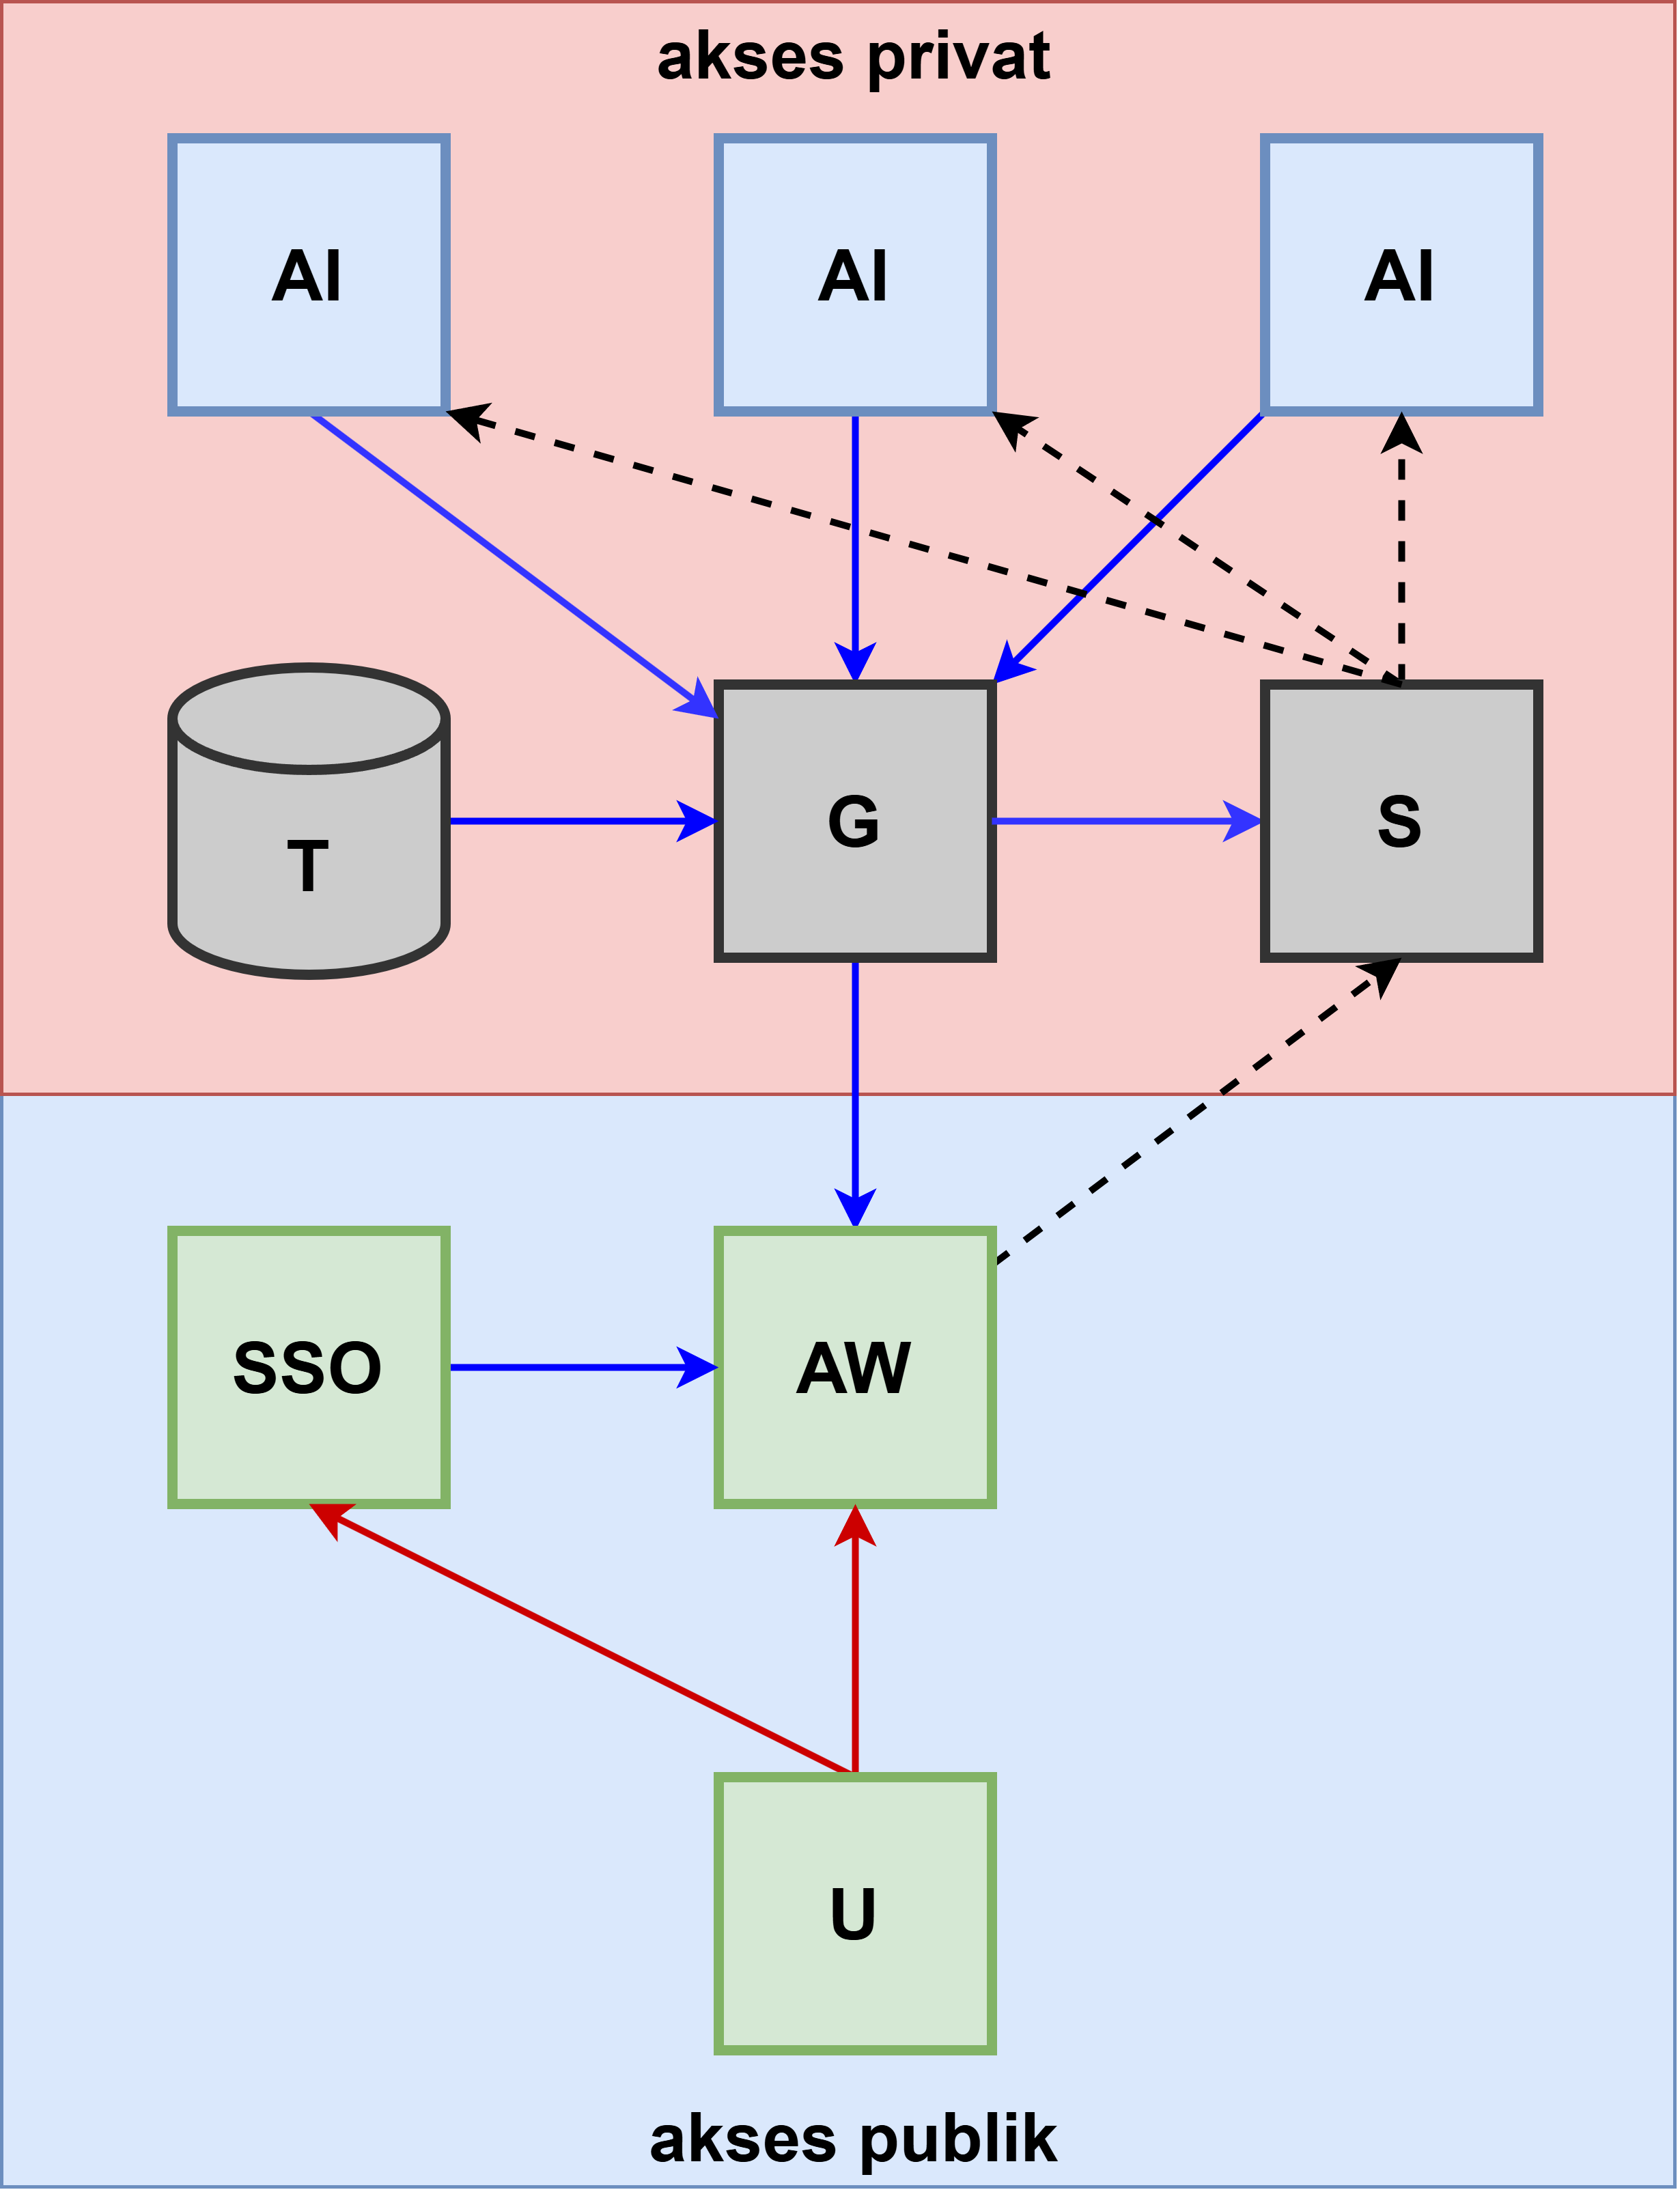
\includegraphics[width=0.5\linewidth]{figures/GambaranUmum.png}
    \caption{Gambaran Umum Arsitektur Sistem}
    \label{fig:GambaranUmum}
\end{figure}
